\documentclass[a4paper]{article}

%% Language and font encodings
\usepackage[utf8]{inputenc}
\usepackage[ngerman]{babel}
\usepackage[T1]{fontenc}
\usepackage{caption}

%% Sets page size and margins
\usepackage[a4paper,top=3cm,bottom=2cm,left=3cm,right=3cm,marginparwidth=1.75cm]{geometry}

%% Useful packages
\usepackage{amsmath}
\usepackage{graphicx}
\usepackage[style=nature]{biblatex}
\usepackage[colorinlistoftodos]{todonotes}
\usepackage[colorlinks=true, allcolors=blue]{hyperref}
\usepackage{float}

% für tabellen
\usepackage{booktabs}

% für Gradzeichen
\usepackage{siunitx}

\addbibresource{references.bib}

\title{Praktikum Neurobiologie - Protokoll 4}

\author{Cedric Laier, Tilman Mehl}


\begin{document}
%Titelpage Modell: https://www.latextemplates.com/template/formal-book-title-page
\begin{titlepage} % Suppresses headers and footers on the title page

	\centering % Centre everything on the title page
	
	\scshape % Use small caps for all text on the title page
	
	\vspace*{\baselineskip} % White space at the top of the page
	
	%------------------------------------------------
	%	Title
	%------------------------------------------------
	
	\rule{\textwidth}{1.6pt}\vspace*{-\baselineskip}\vspace*{2pt} % Thick horizontal rule
	\rule{\textwidth}{0.4pt} % Thin horizontal rule
%	{\LARGE THE BIG BOOK\\ OF\\ \LaTeX ~TEMPLATES\\} % Title
	\vspace{0.75\baselineskip} % Whitespace above the title
	{\LARGE Flügelstreckrezeptor der Heuschrecke} {\\Protokoll zum Praktikum Neurobiologie für Bioinformatiker\\ am 28.01.2019} % Title

	
	\vspace{0.75\baselineskip} % Whitespace below the title
	
	\rule{\textwidth}{0.4pt}\vspace*{-\baselineskip}\vspace{3.2pt} % Thin horizontal rule
	\rule{\textwidth}{1.6pt} % Thick horizontal rule
	
	\vspace{2\baselineskip} % Whitespace after the title block
	
	\vspace{2.0\baselineskip} % Whitespace before the editors

{\LARGE Gruppe 2}
\vspace{2.5\baselineskip} \\
	
{\LARGE Autoren:}
\begin{itemize}
\item Cedric Laier - \textit{cedric.laier@fu-berlin.de}
\item Tilman Mehl - \textit{tilmanmehl@zedat.fu-berlin.de}
\end{itemize}
\vspace{2.5\baselineskip}

{\LARGE Lehrveranstalter:}
\begin{itemize}
\item  Peter Robin Hiesinger
\item Matthias Wernet
\end{itemize}
\vspace{2.5\baselineskip}

{\LARGE Tutoren:}
\begin{itemize}
\item Lisa
\item Johannes
\item Claudia
\end{itemize}
	
\end{titlepage}

%%
%%
%% Kapitel 1: Einleitung
%%
%%

\section{Einleitung}
Inhalt des Praktikumstages waren Experimente am Streckrezeptor einer Heuschrecke. Betrachtet wurde die Antwort dieses Mechanorezeptors bei Ruhe und unterschiedlichen Erregungszuständen.\\ \\
Mechanorezeptoren sind Sinneszellen, die auf mechanische Reize reagieren. Der Streckrezeptor der Heuschrecke ist ein phasisch-tonischer Mechanorezeptor, d.h. bei im Ruhezustand sendet der Rezeptor Aktionspotentiale in einer relativ gleichmäßigen (tonischen)  Frequenz. Bei Erregung steigt die Frequenz zunächst stark an (phasischer Teil), und sinkt dann durch Adaption auf einen neuen Ruhewert ab.

%%
%%
%% Kapitel 2: Versuchsaufbau- und durchführung
%%
%%

\section{Versuchsaufbau und -durchführung}

\subsection{Allgemeiner Versuchsaufbau}

In Abbildung \ref{fig:Versuchsaufbau} ist unser Versuchsaufbau für den 4. Praktikumstag zu sehen. 
Bei den für die Experimente verwendeten Geräte handelte es sich um:

\begin{itemize}
    \item Differenzverstärker
    \item Analog-Digital-Wandler
    \item Spike2 (Software)
    \item Auslenkapparatur
    \item Elektroden
    \item Wachsschale
\end{itemize}

\noindent Bei dem Versuchstier handelte es sich um eine von uns präparierte Heuschrecke. Diese wurde vorrab durch eine Kühlung betäubt und anschließend zur Untersuchung vorbereitet. Dabei wurden Kopf und Beine und Darm der Heuschrecke entfernt und durch einen dorsalen Schnitt an der Mittelline geöffnet. Nun wurden zur Befestigung des Präparats zwei Nadeln an der Cutikula entlang durch das Tier gestochen und an der Wachsschale befestigt. Die Flügel wurden abschließend in der Auslenkapparatur befestigt und mit Knetmasse fixiert. Dem fertig präpariertem Objekt wurden nun zwei Elektroden am Meso N1 Nerv angesetzt. Die Elektroden wiederum mit dem Differenzverstärker verbunden und mithilfe von einem zwischengeschalteten Analog-Digital-Wandler zur digitalen Aufbereitung mit Spike2 konnte dann eine Aufzeichnung der Signale durchgeführt werden.

\begin{figure}[H]
    \centering
    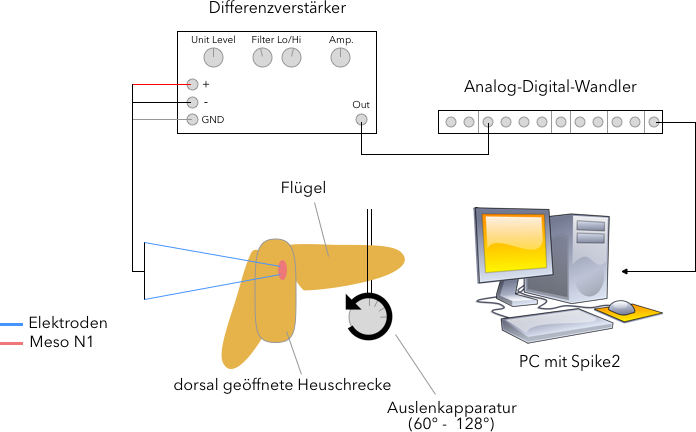
\includegraphics[scale=0.5]{images/Versuchsaufbau__Heuschrecke.png}
    \caption{Versuchsaufbau für alle durchgeführten Experimente}
    \label{fig:Versuchsaufbau}
\end{figure}

\subsection{Versuchsdurchführung}

Für die Versuchsdurchführung wurde bei allen vier Experimenten derselbe Versuchsaufbau  \\ (s. Abbildung  \ref{fig:Versuchsaufbau}) verwendet. 

\subsubsection{Ruhelage}
Bei dem ersten Experiment wurde der Flügel mithilfe der Auslenkapparatur in einen \ang{60} Winkel gebracht. Bei diesem Winkel handelt es sich um die sogenannte Ruhelage des Insektes. Anschließend wurde von uns etwa 120 Sekunden lang eine Signal Aufnahme mit Spike2 durchgefuhrt und anschließend mithilfe des Memory Buffers die Entladungsfrequenz ermittelt.  

\subsubsection{Auslenkung mit Rückführung in die Ruhelage}
Für diesen Teil des Versuchs wurde der Flügel aus der Ruhelage für eine Minute auf \ang{76} Grad ausgelenkt und anschließend für eine Minute wieder in die Ruhelage gebracht. Das jeweilige Antwortverhalten wurde aufgezeichnet.\\
Das Gleiche wurde für die Auslenkwinkel \ang{92}, \ang{108} und \ang{124} durchgeführt.\\
Jede Messung wurde zwei Mal wiederholt und die Mittelwerte für die gemessenen Frequenzen ermittelt.

\subsubsection{Auslenkung ohne Rückführung in die Ruhelage}

In diesem Experiment sind wir ähnlich verfahren wie in Experiment 2.2.2. Die Flügel der Heuschrecke wurden mithilfe der Auslenkapparatur in ihre Ruhepostion gebracht (\ang{60}) und eine Aufzeichnung in Spike2 gestartet. Nun haben wir die den Winkel der Flügel um \ang{16} Grad gesteigert (auf \ang{76}) und mindestens eine Minute die Signale nach der Steigerung aufzeichnen lassen. Anschließend haben wir (ohne in die Ruhelage zurückzukehren) die Flügel erneut um \ang{16} gesteigert (von \ang{76} auf \ang{92}) und erneut mindestens eine Minute Signale aufgezeichnet. Diese Schritte wiederholten wir noch für eine Steigerung von \ang{92} auf \ang{108} und von \ang{108} auf \ang{124}. Abschließend für den Durchlauf wurden die Flügel von \ang{124} auf \ang{60} zurückgeführt und eine fünf minütige Ruhephase eingelegt. Der gesammte genannte Vorgang wurde von uns zwei weitere Male wiederholt, worduch wir am Ende drei Wiederholungen des Experimentes hatten und auswerten konnten. 

\subsubsection{Pronation und Supination}

Bei dem Experiment zur Beobachung der Signal bei der Pronation und Supination wurde die Auslenkapparatur vom Flügel gelöst. Anschließend wurde eine Spike2 Aufnahme gestartet und währenddessen von uns mithilfe einer Pinzette der Flügel der Heuschrecke an ihrer Längsachse erst mit der Flügel-Vorderkante nach unten (Pronation) und dann mit der Flügel-Vorderkante nach oben (Supination) gedreht und die dadurch resultierenden Signale beobachtet.

%%
%%
%% Kapitel 3: Ergebnisse
%%
%%

\section{Ergebnisse}

\subsection{Ruhelage}

Bei der in Abbildung \ref{fig:A2} zu sehenden Aufzeichnung handelt es sich um einen Messzeitraum von 120 Sekunden. Jeder abgebildete blaue Balken entspricht der Hertz Anzahl über 10 Sekunden. Sichtbar zu erkennen ist, dass die Frequenz über den gesamten Zeitraum relativ geleichmäßig ist. Einzelne Spikes sind höchstwahrscheinlich auf Störsignale zurückzuführen.

\begin{figure}[H]
    \centering
    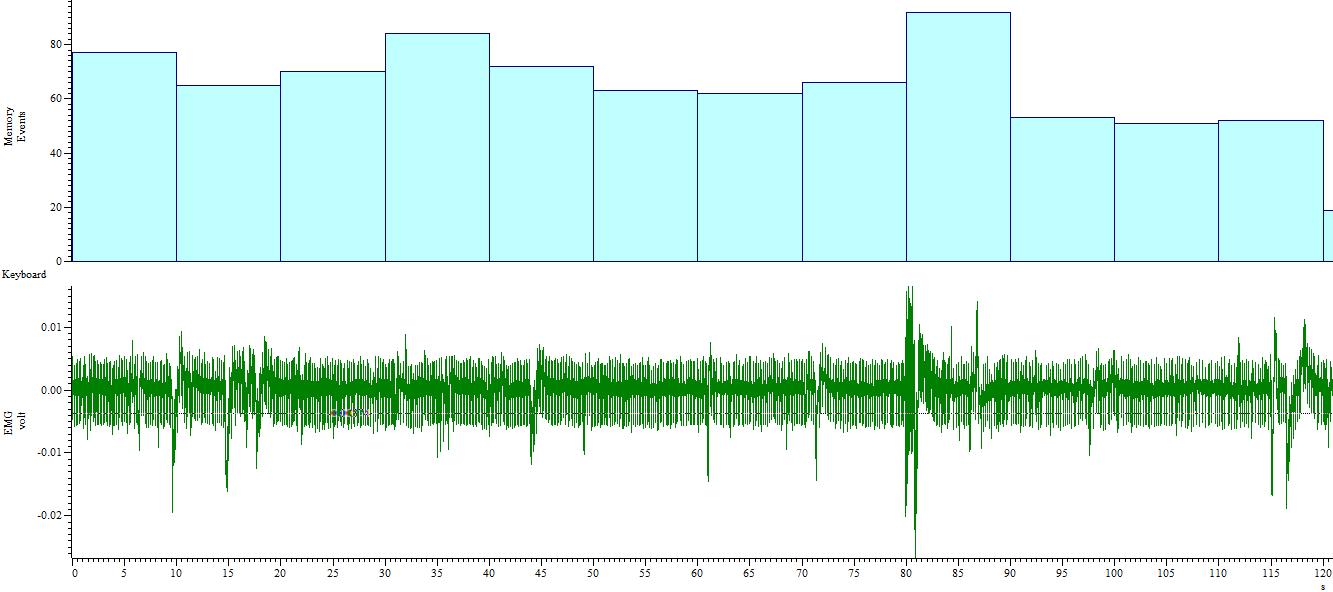
\includegraphics[scale=0.35]{images/A1_Messung.PNG}
    \caption{120 Sekunden Aufzeichnung der Frequenzen in der Ruhelage}
    \label{fig:A2}
\end{figure}

\noindent Ein blauer Balken in Abbildung \ref{fig:A2} entspricht der Anzahl von Events pro 5 Sekunden. Um den Hertz Wert zu ermitteln, haben wir die Event Anzahl durch die Sekunden geteilt, wordurch wir einen Hertz Mittelwert bilden konnten.    
Die anschließend von uns ermittelten Entladungsfrequenz betrug für dieses Experiment ungefähr \fbox{7 Hz}.


\subsection{Auslenkung mit Rückführung in die Ruhelage}
In den ersten 5 Sekunden nach Änderung der Auslenkung konnte starke Erregung gemessen werden (siehe Abbildung \ref{fig:A2plot1}). Besonders hohe Frequenzen waren bei Auslenkungen von \ang{124}, \ang{60}, und \ang{76} Grad zu erkennen.\\ \\
Bei \ang{76} Grad Auslenkung wurde im Zeitraum von 5 bis 10 Sekunden ein starker Abfall der Frequenz beobachtet. In den darauffolgenden 50 Sekunden stieg die Frequenz wieder an und näherte sich der Frequenz der Ruheauslenkung.\\ \\
Bei \ang{92} Grad Auslenkung wurde im Zeitraum von 5 bis 10 Sekunden ein starker Abfall der Frequenz beobachtet. In den folgenden 20 Sekunden steig die Frequenz wieder leicht an, und senkte sich in den nächsten 30 Sekunden auf das Niveau der Frequenz der Ruheauslenkung.\\ \\
Bei \ang{108} Grad Auslenkung nahm die Frequenz nach der initialen Erregung stetig ab und näherte sich der Frequenz der Ruheauslenkung an.\\ \\
Bei \ang{124} Grad Auslenkung wurde nach der initialen Erregung ein starker Abfall und danach eine stetige Abnahme der Frequenz beobachtet, die deutlich unter der Frequenz der Ruheauslenkung lag.
\begin{figure}[H]
\centering
    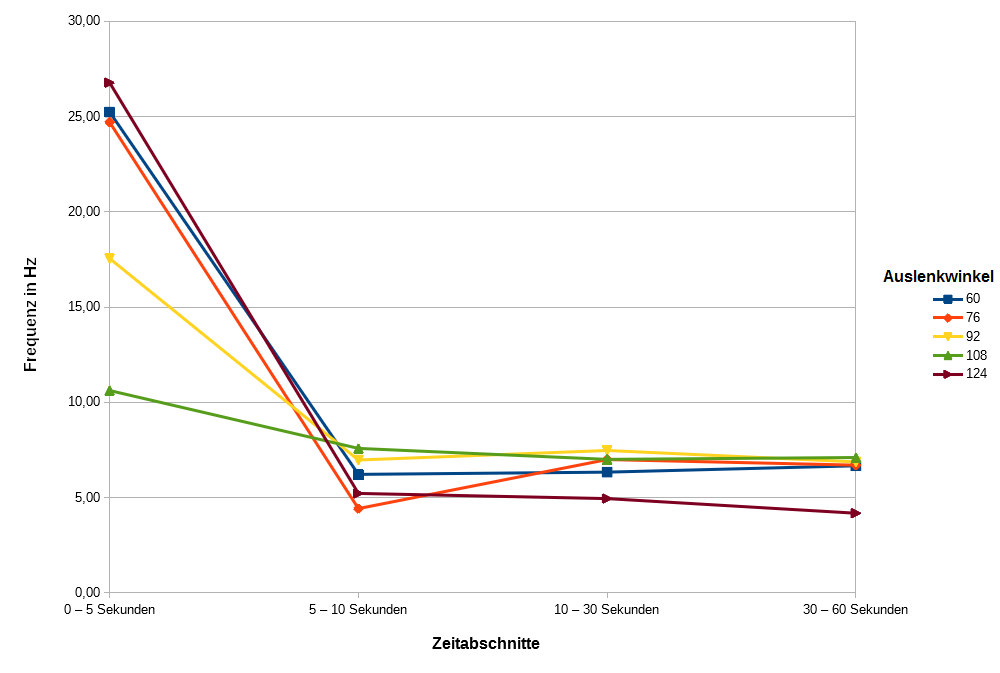
\includegraphics[width=\textwidth]{images/a2plot1.png}
    \caption{Mittelwerte der zu den Auslenkwinkeln gemessenen Frequenzen über die Zeit}
    \label{fig:A2plot1}
\end{figure}
\noindent Die Standardabweichungen der Auslenkwinkel wurden der Übersichtlichkeit halber nicht in im Diagramm aufgeführt. Sie lauten:
\begin{table}[H]
    \centering
    \caption{Standardabweichungen je Auslenkwinkel und Zeitraum}
    \begin{tabular}{c|c|c|c|c|c}
         Auslenkwinkel & 0-5s & 5-10s & 10-30s & 30-60s & Gesamtzeitraum \\
         \hline
         \ang{60} & 10.979 Hz & 1.503 Hz & 1.370 Hz & 1.735 Hz & 9.892 Hz \\
         \ang{76} & 5.119 Hz & 1.578 Hz & 0.788 Hz & 1.089 Hz & 8.827 Hz \\
         \ang{92} & 12.463 Hz & 1.007 Hz & 2.194 Hz & 0.777 Hz & 7.197 Hz \\
         \ang{108} & 5.032 Hz & 2.121 Hz & 2.691 Hz & 2.332 Hz & 3.182 Hz \\
         \ang{124} & 13.144 Hz & 0.757 Hz & 2.351 Hz & 0.344 Hz & 11.478 Hz \\
    \end{tabular}
    \label{tab:A2_sd}
\end{table}
\noindent Die Messungen der phasischen und tonischen Kennlinien ergaben eine deutlich höhe Frequenz für die phasische Antwort (siehe Abbildung \ref{fig:mA2plot2}.\\
Bei der phasischen Anwort wurde mit steigendem Auslenkwinkel zunächst ein starker Abfall beobachtet, für \ang{124} Grad dann wieder ein starker Anstieg über das Niveau der phasischen Antwort bei \ang{60} Grad.\\
Mit Anstieg des Auslenkwinkels stieg auch die tonische Frequenz schwach an, fiel jedoch für \ang{124} Grad unter das Niveau der tonischen Antwort bei \ang{60} Grad.
\begin{figure}[H]
    \centering
    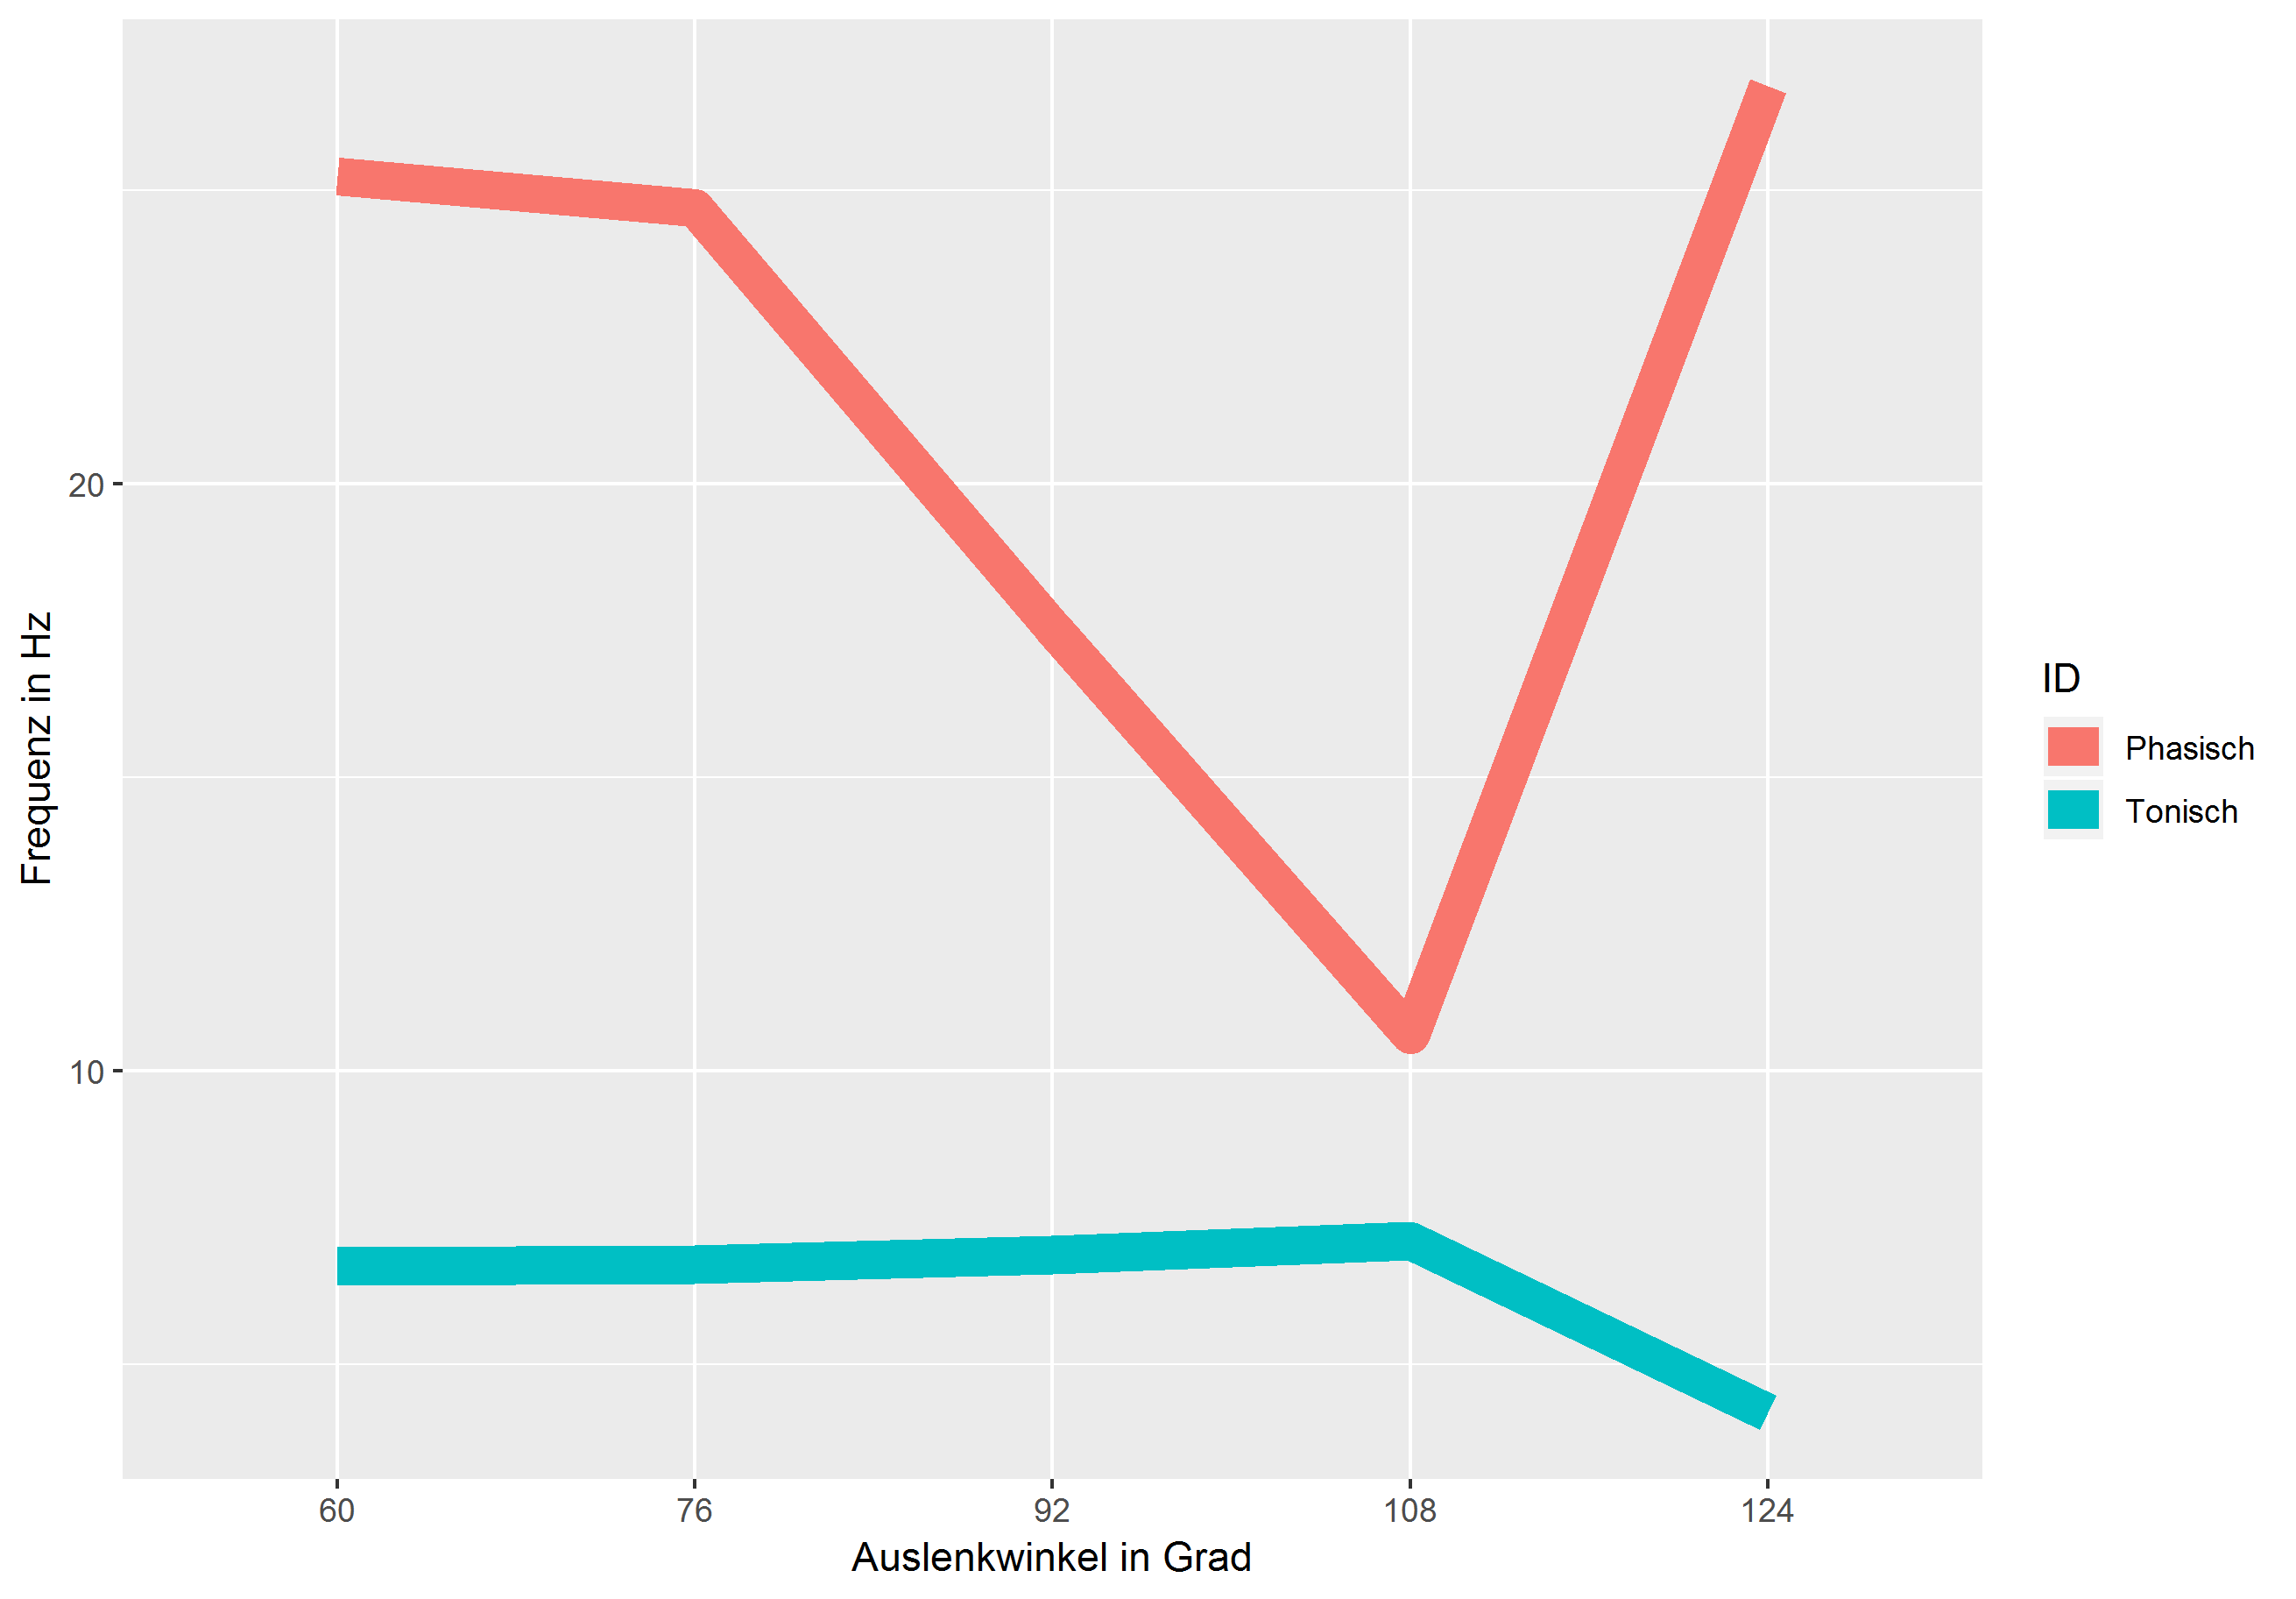
\includegraphics[scale=0.8]{images/a2plot2.png}
    \caption{Phasische und Tonische Kennlinie}
    \label{fig:mA2plot2}
\end{figure}

\newpage
\subsection{Auslenkung ohne Rückführung in die Ruhelage}

In den nachfolgenden Abbildungen 2 - 6 sind die Aufzeichnungen vom ersten Messdurchgang zu sehen. Zur Auswertung wurden die Aufzeichnung jeder Flügelauslenkung in einzelne Teilbereiche eingeteilt. Die erste Entladungsfrequenzmessung erfolgte über den Zeitraum von 0s - 5 Sekunden nach der Auslenkung, die zweite von 5s - 10 Sekunden, die dritte von 10s - 30 Sekunden und der vierte Messung erfolgte für den Zeitraum 30s - 60 Sekunden. \\ \\
Diese Messungen der Teilbereiche wurden dann bei jeder Auslenkungsaufzeichnung durchgeführt und abschließend in der Tabelle \ref{tab:A3} eingetragen. Ein blauer Balken in den Abbildungen bildet dabei die Frequenz in Hertz über den jeweiligen Zeitraum von einer Sekunde ab. 

\vspace{4.5\baselineskip} \\
\begin{figure}[H]
    \centering
    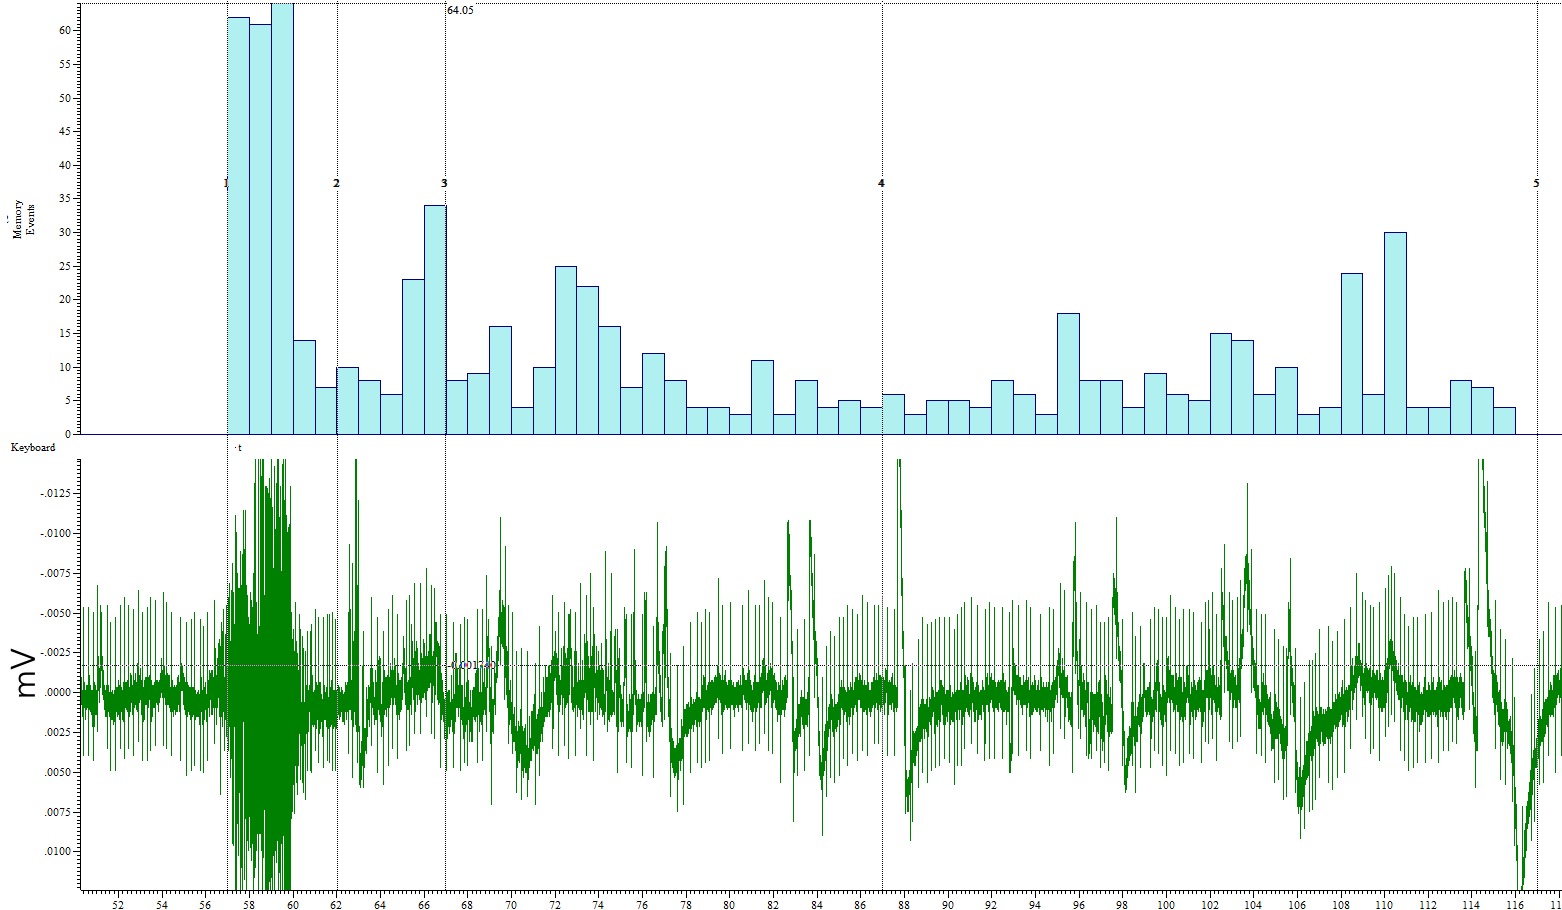
\includegraphics[scale=0.27]{images/A3_60-76Grad.PNG}
    \caption{\label{fig:A3_1}Flügel-Auslenkung von \ang{60} auf \ang{76}}
\end{figure}

\vspace{2.5\baselineskip} \\
\begin{figure}[H]
    \centering
    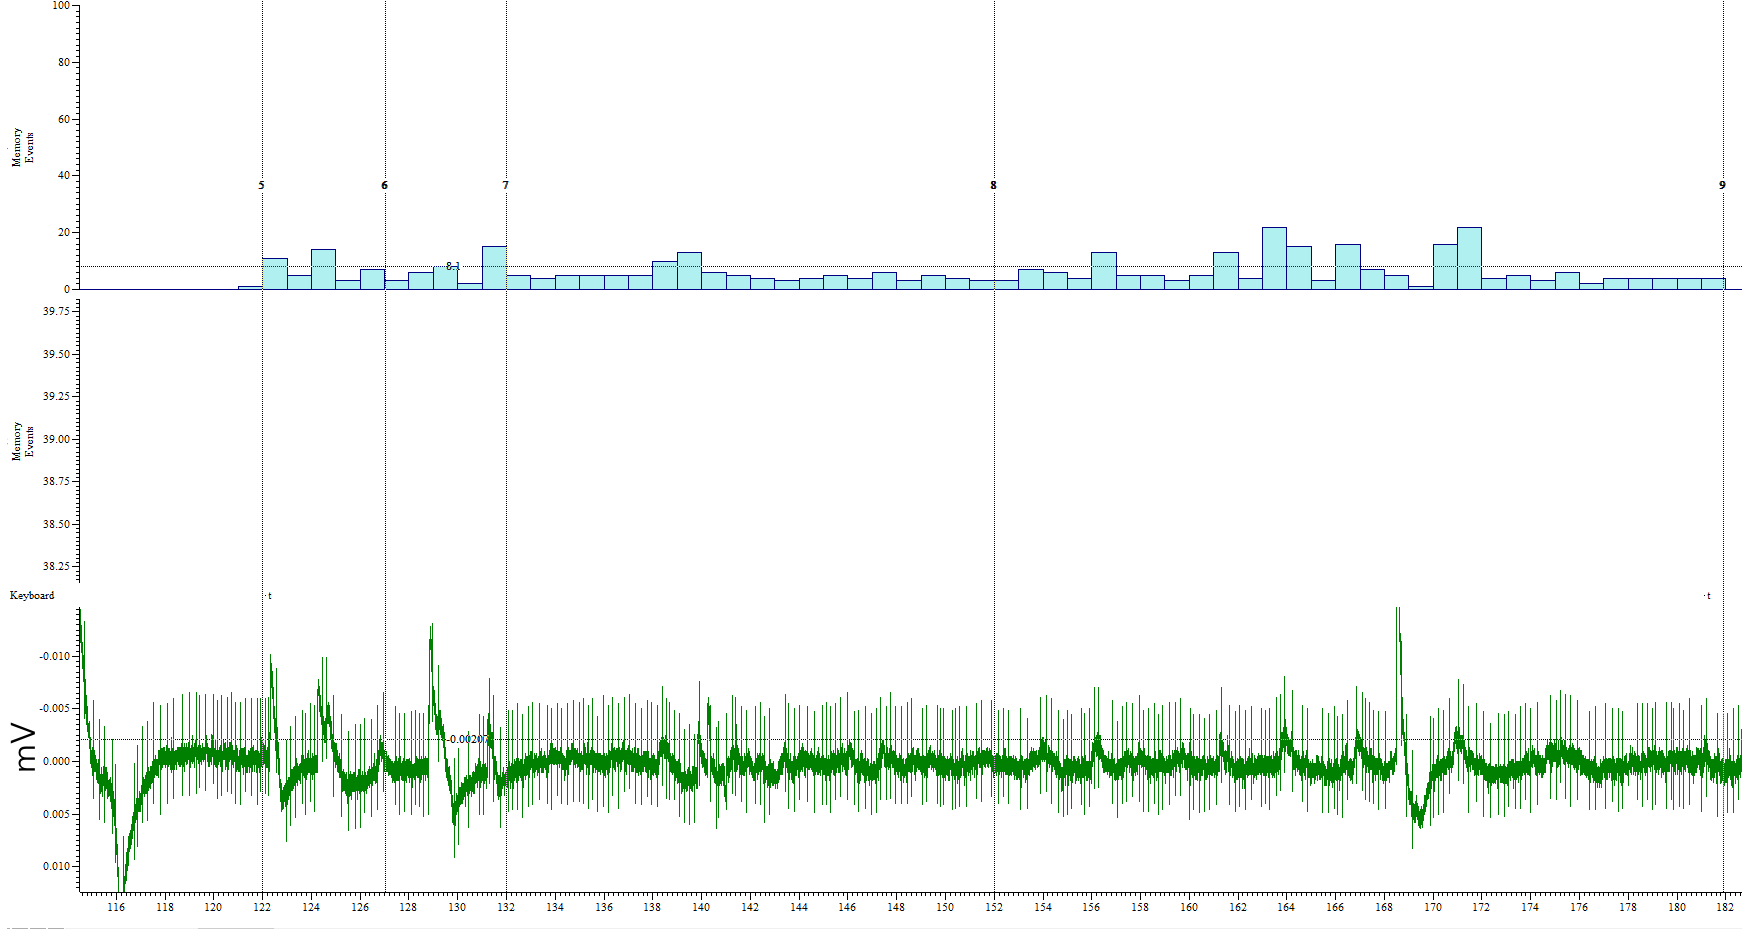
\includegraphics[scale=0.25]{images/A3_76-92Grad.PNG}
    \caption{\label{fig:A3_2}Flügel-Auslenkung von \ang{76} auf \ang{92}}
\end{figure}

\vspace{4.5\baselineskip} \\
\begin{figure}[H]
    \centering
    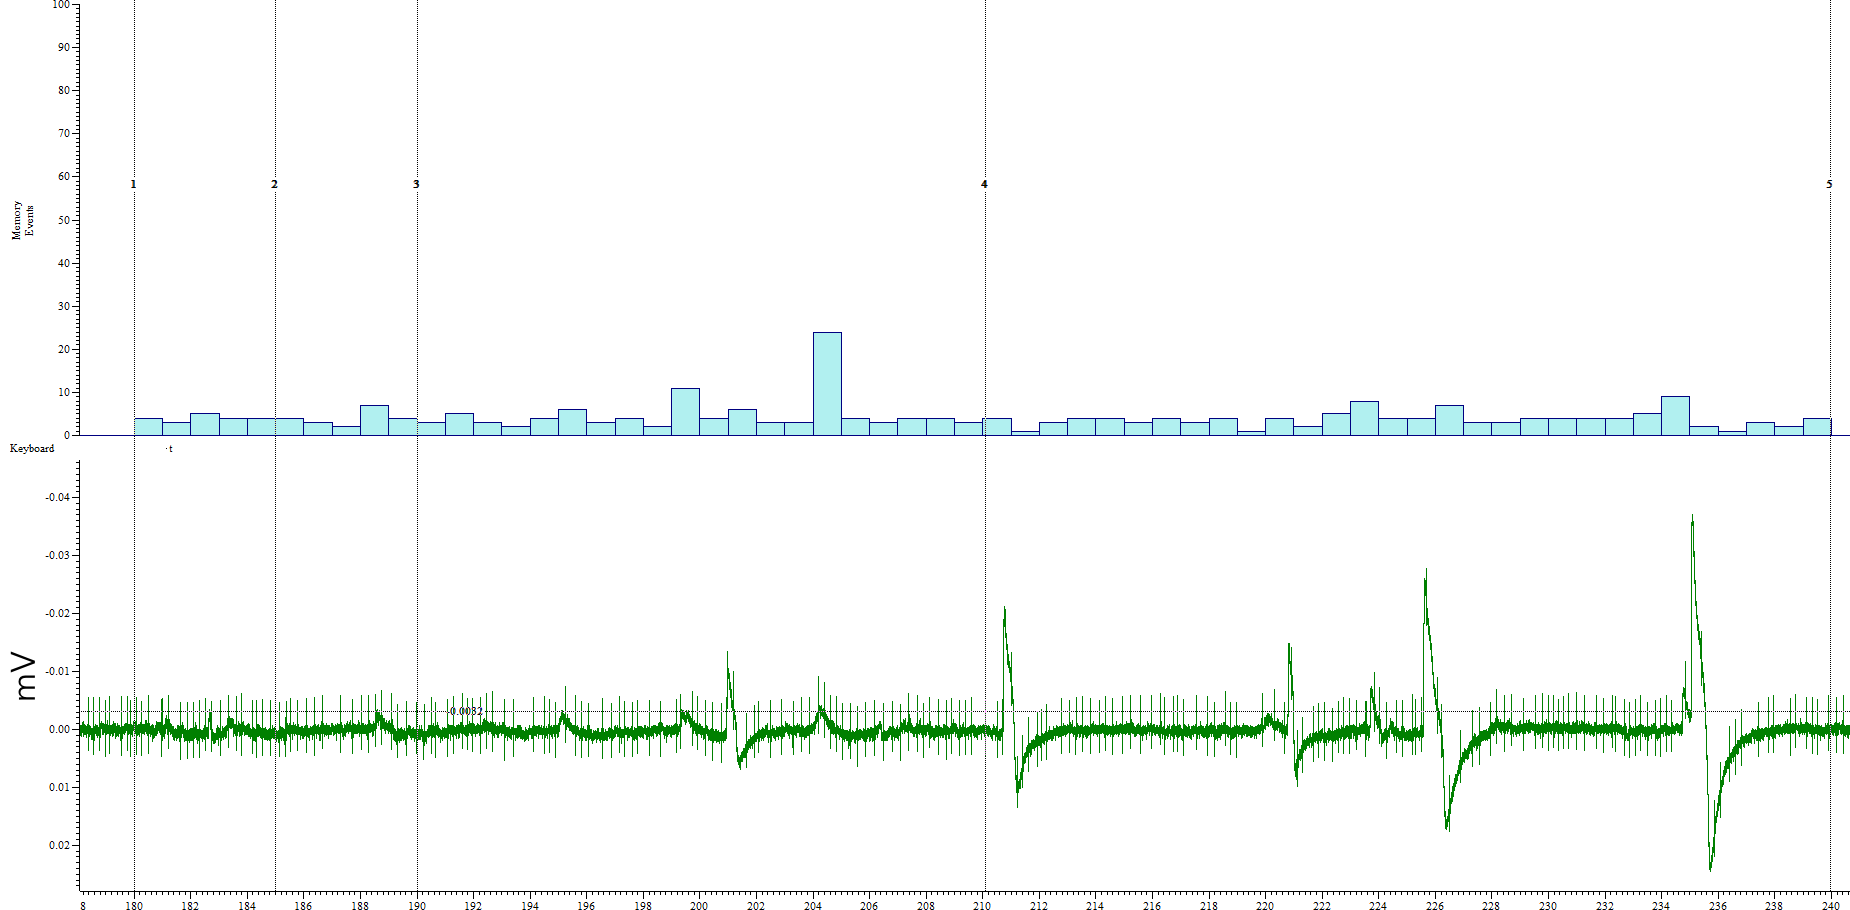
\includegraphics[scale=0.245]{images/A3_92-108Grad.PNG}
    \caption{\label{fig:A3_3}Flügel-Auslenkung von \ang{92} auf \ang{108}}
\end{figure}

\vspace{2.5\baselineskip} \\
\begin{figure}[H]
    \centering
    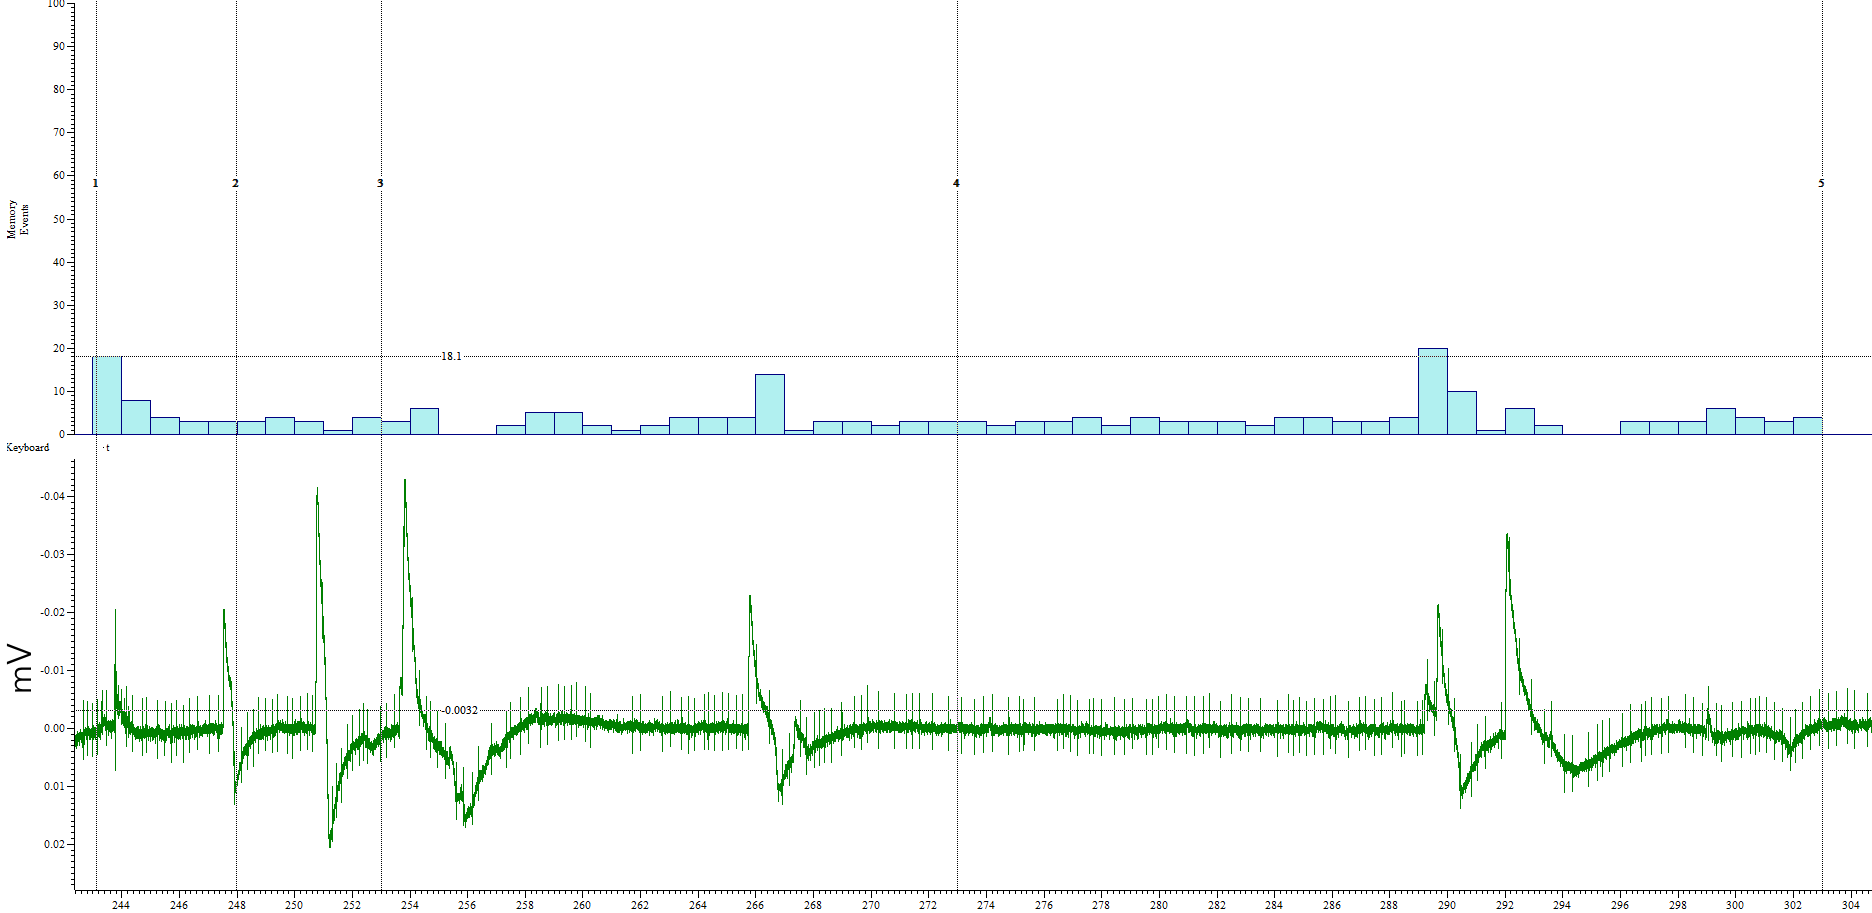
\includegraphics[scale=0.25]{images/A3_108-124Grad.PNG}
    \caption{\label{fig:A3_4}Flügel-Auslenkung von \ang{108} auf \ang{124}}
\end{figure}

\vspace{4.5\baselineskip} \\
\begin{figure}[H]
    \centering
    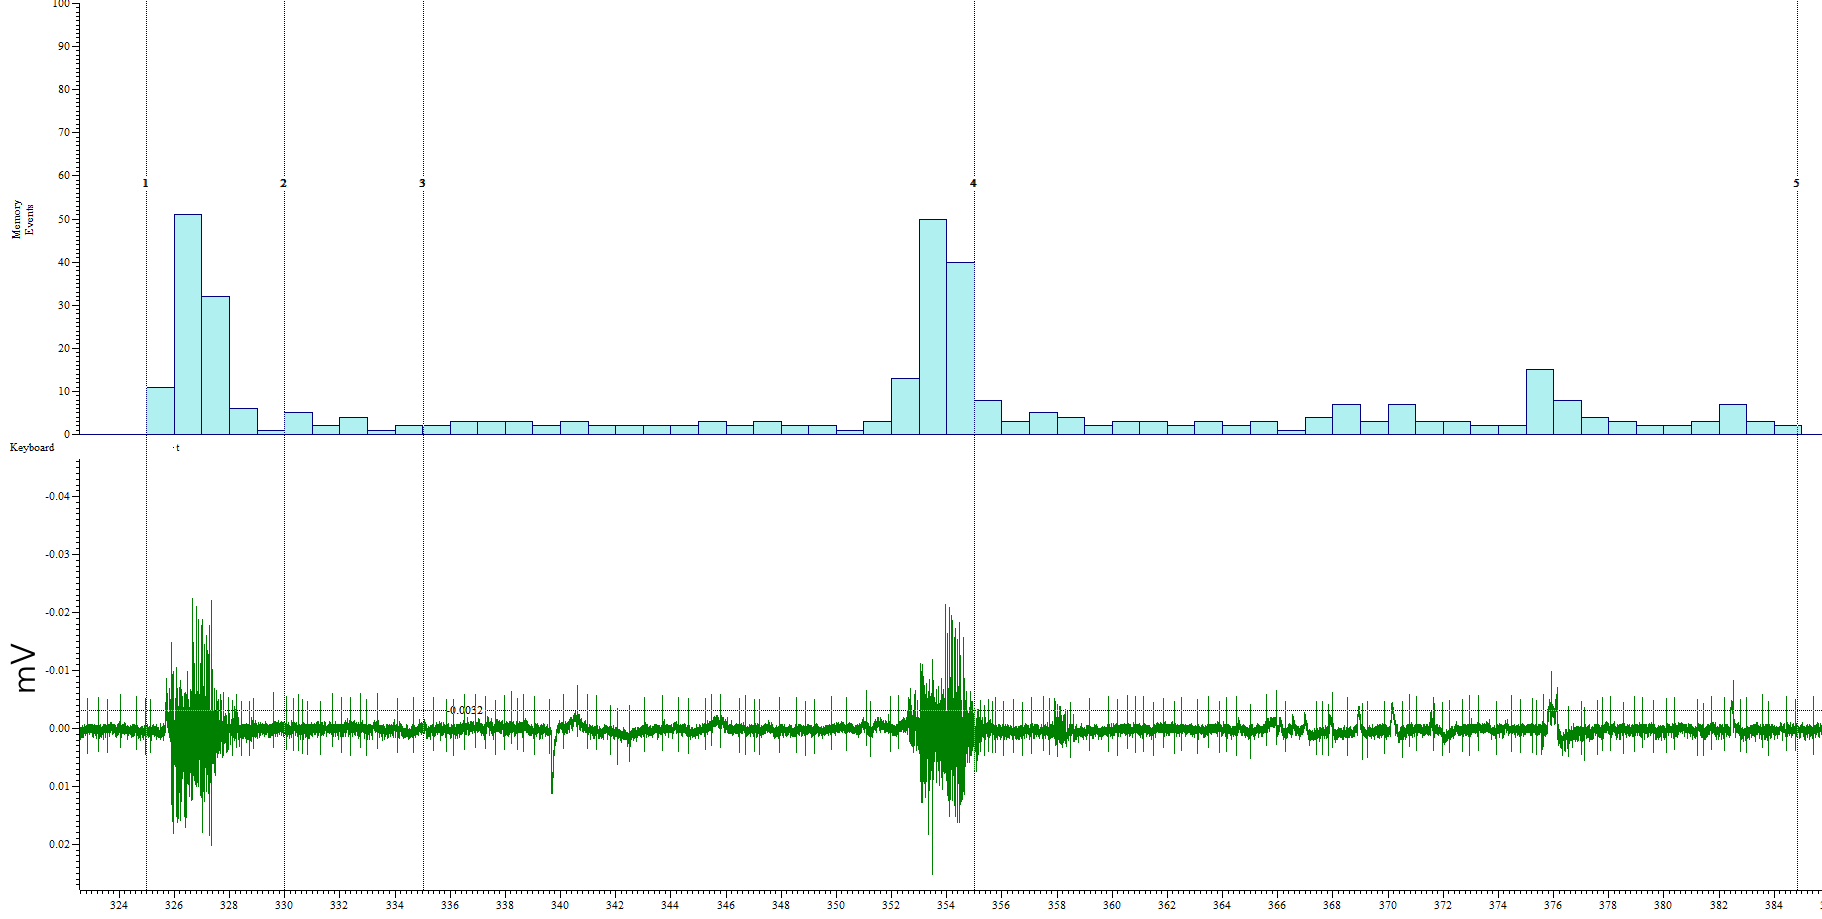
\includegraphics[scale=0.26]{images/A3_124-60Grad.PNG}
    \caption{\label{fig:A3_5}Flügel-Rückführung von \ang{124} zurück auf \ang{60}}
\end{figure}

\vspace{2.5\baselineskip} \\

\newpage
\noindent Tabelle \ref{tab:A3} listet die Entladunsfrequenzen der Streckenrezeptoren jeder Auslenkstufe einzelner Teilmesszeiträume über den Gesamtmesszeitraum von 60 Sekunden auf. Bei den eingetragenen Werten handelt es sich um einen Mittelwert aus drei Messdurchläufen. In Kapitel 4.3 wird von uns Rückschluss zu den erzielten Messwerten getroffen.

\vspace{1.5\baselineskip} \\

\begin{table}[H]
\centering
    \begin{tabular}{@{}cllll@{}}
    \toprule
        \multicolumn{1}{l}{Auslenkwinkel} & 0s - 5s & 5s - 10s & 10s - 30s & 30s - 60s \\ \midrule
        \ang{60} \rightarrow \ang{76}                                & \multicolumn{1}{c}{36 Hz}         & \multicolumn{1}{c}{16 Hz}          & \multicolumn{1}{c}{9 Hz}           & \multicolumn{1}{c}{7 Hz}           \\
        \ang{76} \rightarrow \ang{92}                               & \multicolumn{1}{c}{9 Hz}         & \multicolumn{1}{c}{8 Hz}          & \multicolumn{1}{c}{6 Hz}           & \multicolumn{1}{c}{5 Hz}      \\
        \ang{92} \rightarrow \ang{108}                               & \multicolumn{1}{c}{5 Hz}         & \multicolumn{1}{c}{4 Hz}          & \multicolumn{1}{c}{4 Hz}           & \multicolumn{1}{c}{4 Hz}      \\
        \ang{108} \rightarrow \ang{124}                               & \multicolumn{1}{c}{7 Hz}         & \multicolumn{1}{c}{6 Hz}          & \multicolumn{1}{c}{5 Hz}           & \multicolumn{1}{c}{4 Hz}      \\
        \ang{124} \rightarrow \ang{60}                               & \multicolumn{1}{c}{20 Hz}         & \multicolumn{1}{c}{4 Hz}          & \multicolumn{1}{c}{4 Hz }           & \multicolumn{1}{c}{3 Hz}      \\ \bottomrule
    \end{tabular}
    \caption{\label{tab:A3}Gemessene Entladungsfrequenzen (Hz) des Streckrezeptors \\ im jeweiligen Messzeitraum}
\end{table}

\subsection{Pronation und Supination}
In Abbildung \ref{fig:A4} ist die Aufzeichnung der Pro- und Supination zu sehen. Leider konnte es uns nicht gelingen, auswertbare Ergebnisse zu erzielen, da wir bei dem Versuch der Flügeldrehung die Halterung der Heuschrecke verschoben, haben wodruch wir anschließend nicht mehr in der Lage waren den Meso N1 Nerv zu treffen um erneut APs aufzuzeichnen.
Unseren erwarteten Ergebnisse nennen wir in Kapitel 4.4.
\vspace{2.5\baselineskip} \\
\begin{figure}[H]
    \centering
    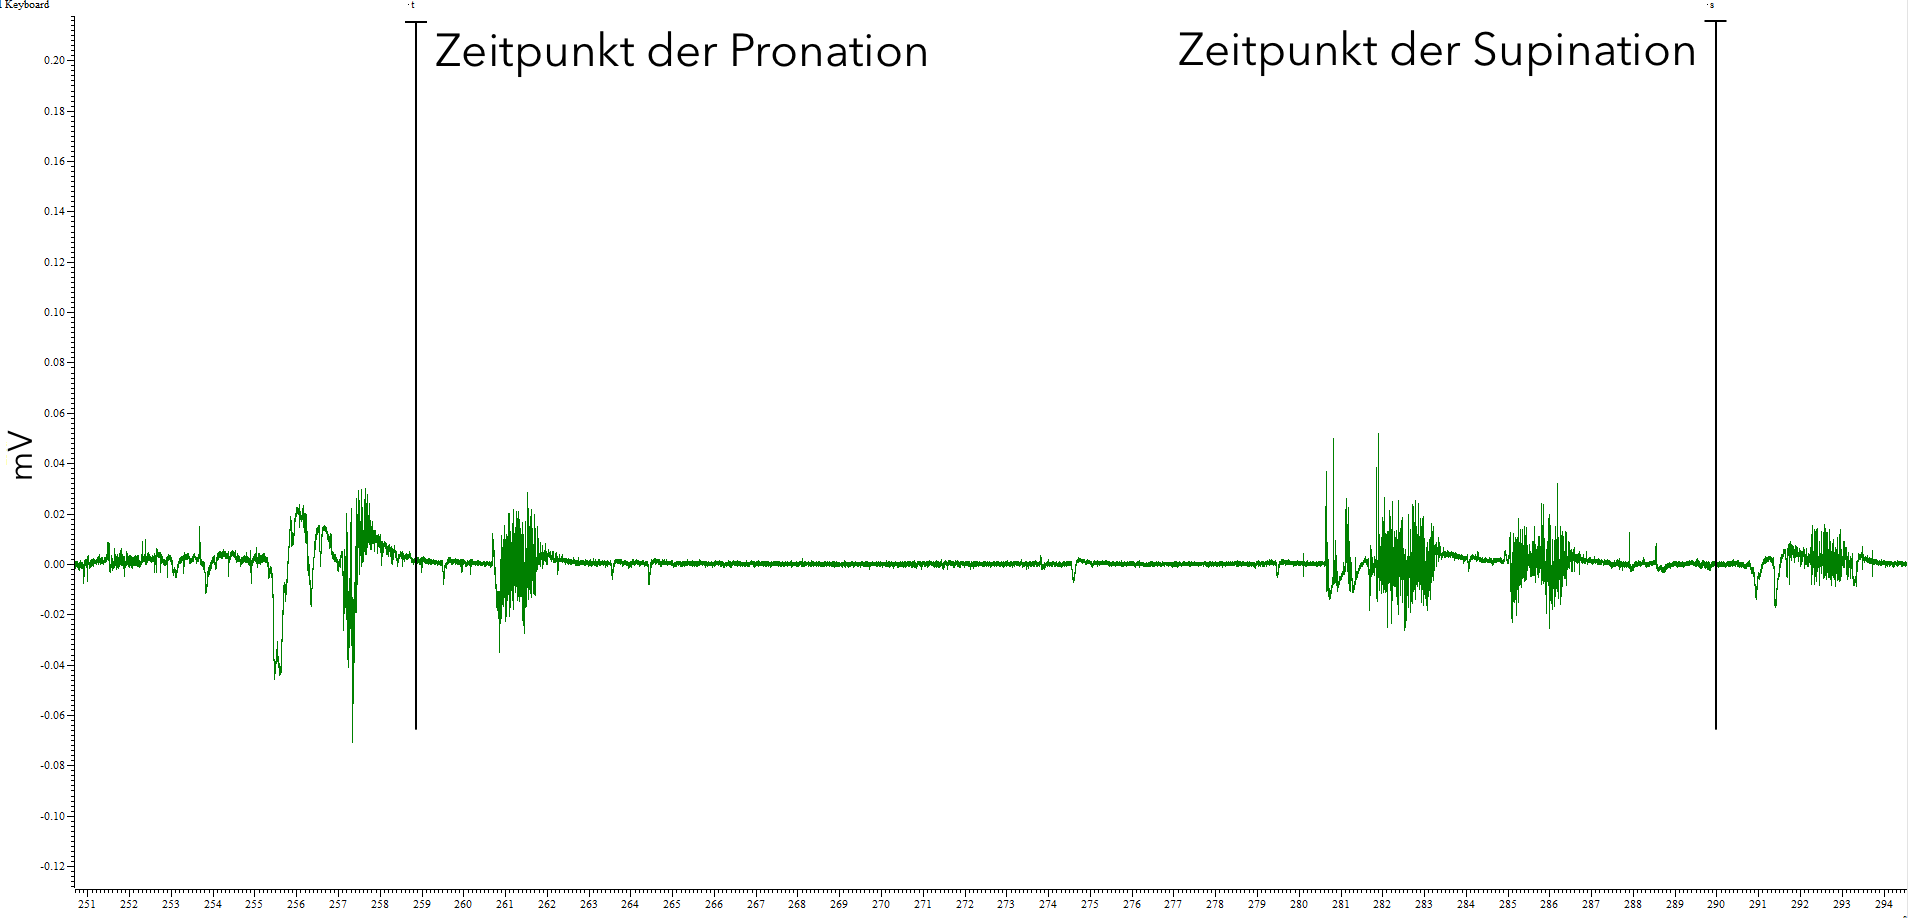
\includegraphics[scale=0.2]{images/A4_Messung.png}
    \caption{\label{fig:A4} Aufzeichnung der Flügeldrehung an ihrer Längsachse \\ (Pronation und Supination)}
\end{figure}
\vspace{2.5\baselineskip} \\

%%
%%
%% Kapitel 4: Diskussion
%%
%%

\newpage
\section{Diskussion}

\subsection{Ruhelage}
Wie zu erwarten konnte bei dem Streckrezeptor in Ruhelage eine gleichmäßige tonische Antwort gemessen werden.

\subsection{Auslenkung mit Rückführung in die Ruhelage}
Wie zu erwarten ist der die Erregung in den ersten Sekunden nach Änderung der Auslenkung am stärksten (phasische Antwort).\\
Leider konnten bei \ang{108} Grad Auslenkung nur einmal die phasische Erregung aufgezeichnet, daher weichen die gemessenen Daten stark von der erwarteten Frequenz ab. Bei \ang{92} Grad Auslenkung konnte die phasische Erregung nur zweimal aufgezeichnet werden, daher auch hier ein niedriger Wert als erwartet.\\
Nach der initialen Erregung ist wie erwartet nur noch die tonische Antwort zu messen, die sich, bedingt durch Adaption an den Reiz, der Frequenz der Ruheauslenkung annähert.\\ \\
Leider kann aus den Messungen zur phasischen Kennlinie kein eindeutiger Schluss gezogen werden, da die Messergebnisse fehlerhaft waren. Zu erwarten gewesen wäre eine stärkere phasische Antwort bei stärkerer Auslenkung.\\

\subsection{Auslenkung ohne Rückführung in die Ruhelage}

Tabelle \ref{tab:A3} zeigt deutlich, dass es bei der initalen Bewegung (Ruhelage \ang{60} zu einem Winkel von \ang{76}) des Flügels in den ersten 5 Sekunden zu einem hohen Frequenzanstieg kommt. In den folgenden 5 Sekunden fällt die Frequenz um etwa die Hälfte (16Hz) ab und pendelt sich in den kommenden 50 Sekunden bei 9 - 7 Hz ein. Die nachfolgenden Gradsteigerungen jedoch besitzen nur eine geringe initale Frequenzerhöhung. Das lässt vermuten, dass es bei bereits angewinkelten Flügeln keine starke Erhöhung der gefeuerten APs nötig ist. Erst als wird den Flügel aus der \ang{124} Postion in die Ruhepostion zurückführen \ref{60}, kommt es erst wieder zu einer erhöhten Frequenz. Hier ist der Reiz so groß, dass dementsprechend wieder viele Aktionspotentiale in den ersten Sekunden gefeuert werden.

\subsection{Pronation und Supination}
Wie in Kapitel 3.4 bereits erwähnt, waren wir nicht in der Lage aus unseren Messungen einen Rückschluss zu ziehen. Allerdings hätten wir bei dem Experiment erwartet, dass eine sichtbar erhöhte Frequenz bei der Pronation zu sehen gewesen wäre. Bie der Pronation des Flügels handelt es sich um eine Bewegung die tendenziell nicht zum normalen Bewegungsablauf der Heuschrecke gehört, sondern eher in Stress- und Fluchtsituationen eingesetzt wird. Die Supination des Flügels hingegen ist eher in den regulären Bewegungsablauf integriert, da beispielsweise beim Gleiten durch die Luft die Vorderkante des Flügels nach oben ausgerichtet ist. 

\printbibliography

\end{document}